\section{Description}
This method uses stochastic event sets and associated ground motion fields to compute loss curves for each asset contained in an exposure file, as illustrated in the following scheme:  

\begin{figure}[ht]
\centering
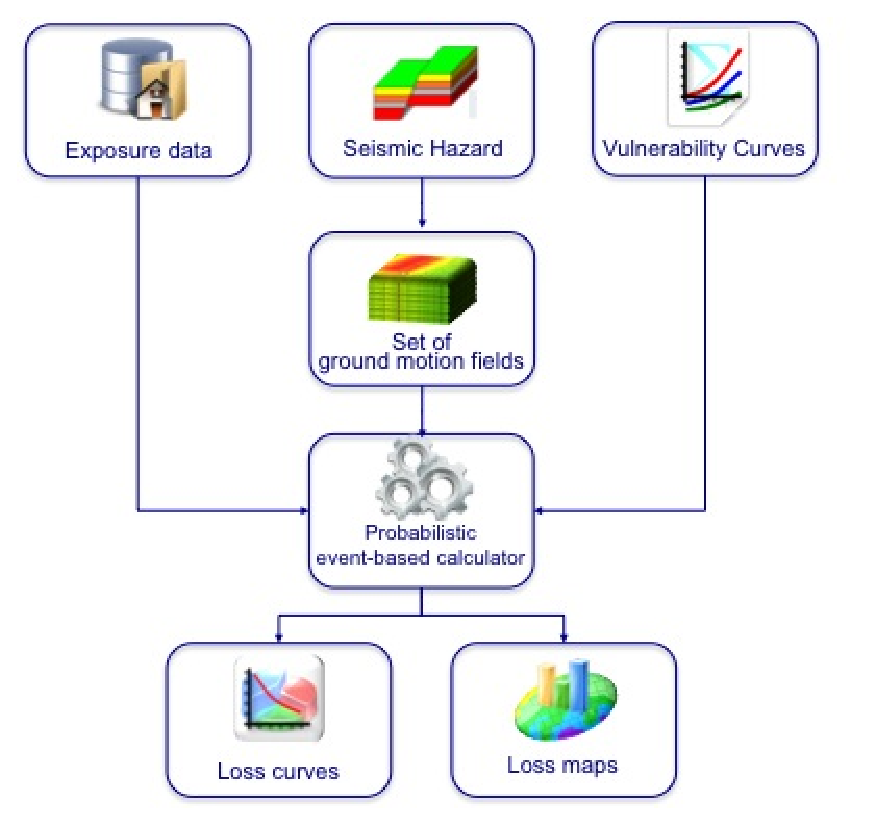
\includegraphics[width=9cm,height=10cm]{./Figures/Part_Risk/Scheme_Prob_calc.eps}
\caption{Architecture of the probabilistic event-based calculator.}
\label{fig:Scheme_Prob_calc}
\end{figure}

For each ground motion field, the intensity measure level at a given site is used to calculate the mean loss ratio using the vulnerability functions for each asset defined in the exposure file. The occurrence distribution of mean loss for a given asset is calculated using all of the ground motion fields, leading to a histogram of loss ratios which is then converted into a cumulative histogram, by calculating the number of cumulative occurrences for each interval of loss ratio. The rate of exceedance of each loss ratio is calculated by dividing the number of cumulative occurrences by the number of stochastic event sets multiplied by the length of each event set. By assuming a Poissionian distribution of the occurrence model, the probability of exceedance of each loss ratio is calculated. 
 
\par \ 

\par
 
If an aggregated loss curve for a portfolio of assets is required, a secondary module is required in order to aggregate the losses from all the assets in the exposure file, per event, before calculating the occurrence distribution of mean loss. If the assets are close enough, it is necessary to generate the ground motion fields taking into account the spatial correlation of ground motion residuals. 

\section{Calculations workflow}



